\subsection{Esquema del servidor}

    El esquema de servidor se basa en el patrón \emph{MVC} (Modelo, Vista, Controlador) que provee \emph{CodeIgniter} con su framework.

    A continuación se muestra un ejemplo del funcionamiento del patrón \emph{MVC} que provee \emph{CodeIgniter}:

        \begin{itemize}
            \item Un usuario lanza una petición contra la siguiente url

                http://www.example.com/clientes/get\_cliente/1

            \item A través del modulo mod\_rewrite se redirige la petición al fichero \emph{index.php} de CodeIgniter, el cual se encarga de analizar la petición siguiendo el siguiente flujo de trabajo:

            \begin{figure}[H]
                \centering
                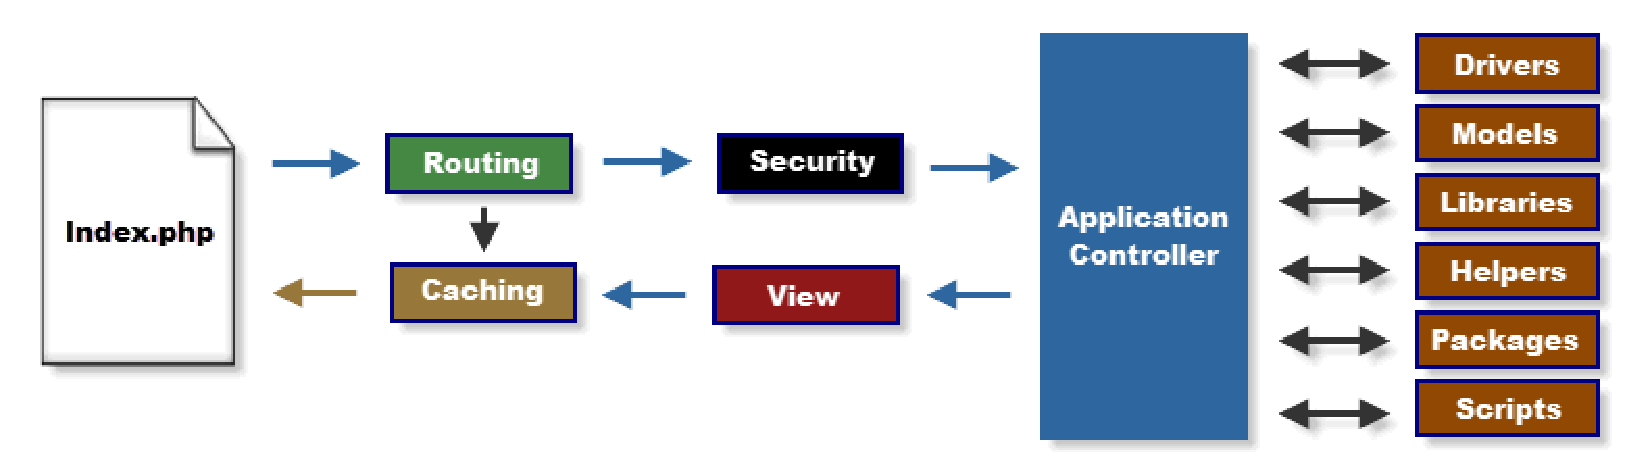
\includegraphics[keepaspectratio,width=0.9\textwidth]{flujo-trabajo-codeigniter.eps}
                \caption{Flujo de trabajo de CodeIgniter}\label{fig:flujo-trabajo-codeigniter}
            \end{figure}

            \item CodeIgniter descompone la URL en la siguiente estructura para conocer a que controlador tiene que pasar la petición, a que función llamar y qué parametros debe pasar.

                http://example.com/[controller-class]/[controller-method]/[arguments]

            Siendo para nuestro ejemplo los siguientes valores:

                \begin{itemize}
                    \item Controller class: clientes
                    \item Controller method: get\_cliente
                    \item Arguments: 1
                \end{itemize}
        \end{itemize}

    Los controladores son los encargados de procesar la petición, cargar tantas librerías, modelos... como necesiten para finalmente devolver un resultado.

    \subsubsection{Extendiendo el core de CodeIgniter}

    CodeIgniter al cargarse intenta buscar los sisguientes ficheros de sistema en la carpeta \emph{application/core}, esta funcionalidad permite sobreescribir algunas de las funcionalidades para ampliarlas.

    En el proyecto se han creado dos nuevos controladores para ampliar la funcionalidad del controlador por defecto de CodeIgniter:

    \begin{itemize}
        \item MY\_Controller

        Extiende de \emph{CI\_Controller} y se encarga de:

            \begin{itemize}
                \item Cargar la librería \emph{login\_auth} si no se están ejecutando los tests unitarios
                \item Ofrecer los siguientes métodos para renderizar la respuesta (\emph{\_renderJson}, \emph{\_renderXml}, \emph{\_renderToVar}, \emph{\_render})
            \end{itemize}

        \item MY\_Controller\_User

        Extiende de \emph{MY\_Controller} y únicamente se encarga de validar en el constructor que el usuario está logueado en el sistema, en caso de no estarlo, redirije a la Home pública.
    \end{itemize}

    \subsubsection{Esquema de controladores}

El esquema de controladores se pueden dividir en dos partes; aquellos que permiten el acceso a la web (la aplicación web los utiliza para renderizar la página) y controlan la sesión del usuario; y aquellos que funcionan como una API \emph{RESTful}, solamente devuelven objetos \emph{JSon}.

Controladores de acceso web

    \begin{itemize}
        \item home.php

            Se encarga de renderizar la parte pública de la web y controlar las acciones de registro de usuario, recordatorio de contraseña y acceso a la zona privada de usuario.

        \item tablon.php

            Se encarga de renderizar el esqueleto de la parte privada de usuario, de controlar que está logueado en el sistema y de permitir salir de su sesión.
    \end{itemize}

Controladores de API \emph{RESTful}

    \begin{itemize}
        \item fridge.php

            Se encarga de procesar las solicitudes para manejar los frigoríficos del usuario y los productos que contienen, así como sus compras.

        \item supermercado.php

            Se encarga de procesar las solicitudes para manejar los supermercados y los productos que contienen.

        \item api.php

            Proporciona una serie de funciones accesibles desde el exterior para permitir al lector comunicarse con el servidor. Por ejemplo, añadir un producto al frigorífico del usuario.

    \end{itemize}

    \subsubsection{Esquema de librerías}

La única restricción que se ha encontrado en CodeIgniter para hacer tests unitarios es que los controladores no se pueden cargar para hacerles pruebas unitarias. Por ello, toda la funcionalidad compleja se traslada a una librería específica la cual tiene sus tests unitarios.

De esta manera el controlador, no necesita de tests unitarios ya que actua como mediador entre el cliente y las librerías.

Se han implementado las siguientes librerías en el sistema:

    \begin{itemize}
        \item Login\_auth\_library.php

            Esta librería es la más crucial a la hora de aportar seguridad ya que se encarga de validar los datos de un usuario cuando intenta acceder al sistema; además de controlar el registro de los usuarios, la recuperación de contraseñas y la opción para salir de una cuenta; destruyéndo la sesión del usuario.

            Se ha utilizado la función nativa \emph{password\_hash} que ofrece \emph{PHP} para crear el Hash de la contraseña que guardaremos en base de datos. Esta función solo funciona en versiones de \emph{PHP 5.5.0} o superiores, si es inferior se utiliza la función \emph{crypt}.

            El algoritmo empleado para hashear con la función \emph{password\_hash} es \emph{BCrypt}. Este algoritmo se considera seguro y perdurable en el tiempo ya que puede establecer el coste de computación para obtener el hash, por lo que aunque la potencia de cálculo de las máquinas aumente se puede aumentar el coste de computación, esto hace que en un futuro siga siendo un algoritmo fuerte contra ataques de fuerza bruta.

            Por el contrario, el algoritmo \emph{DES} que utiliza la función \emph{crypt} se considera insegura, ya que el tamaño de clave que emplea solo es de 56 bits,

            La función para obtener el Hash se encarga de comprobar la versión de \emph{PHP}, si es inferior se utiliza la función \emph{crypt} con un \emph{salt}; aún así a día de hoy ya se empieza a considerar inseguro porque utiliza un algoritmo DES \emph{Data Encryption Standard} con un tamaño de clave de 56 bits que permite realizar ataques de fuera bruta para obtener la contraseña en un tiempo relativamente corto.

            A continuación se expone la función para obtener el hash de una contraseña, donde se compara la versión de \emph{PHP} para utilizar uno u otro:

            \begin{lstlisting}
private function get_password_hash($password) {
    $password_hashed = NULL;

    if (strnatcmp(phpversion(),'5.5.0') >= 0) {
        $password_hashed = password_hash($password, PASSWORD_BCRYPT);
    } else {
        // Original PHP code by Chirp Internet: www.chirp.com.au
        // Please acknowledge use of this code by including this header.
        $salt = "";
        $salt_chars = array_merge(range('A','Z'), range('a','z'), range(0,9));
        for($i=0; $i < 22; $i++) {
            $salt .= $salt_chars[array_rand($salt_chars)];
        }
        $password_hashed = crypt($password, sprintf('$2a$%02d$', 7) . $salt);
    }

    return $password_hashed;
}
            \end{lstlisting}

            Además, para evitar ataques de fuera bruta, se ha implementado un sistema que registra los intentos para acceder a una cuenta. Incrementando hasta un máximo de 45 segundo el tiempo entre intentos, y además, al llegar a este máximo a partir del cual se considera que es un ataque de fuerza bruta, en el formulario se incluye un campo de seguridad para que el usuario resuelva (una operación matemática).

        \item My\_PHPMailer.php

            Esta librería permite el envío de correos electrónicos a través de SMTP ó, si el servidor no lo soporta, utilizando el método \emph{send\_mail}. Para funcionar se carga la librería \emph{PHPMailer}, esta librería implementa funcionalidades para el envío de email como el soporte para el envío de adjuntos o el disponer de una implementación de un servidor \emph{SMTP} para entornos donde no se dispone de un servidor de correos local.

        \item Lector\_library.php

            Esta librería nos permite crear y asociar los lectores físicos que se dispongan.

            Para asociar un lector se generan dos códigos de barras que deben ser escaneados en el tiempo de una hora; tiempo en el que están activos. El formato de los códigos de barras es el siguiente:

            \begin{itemize}
                \item Primer código de barras

                    Está formado por la suma del identificador del usuario más la fecha unix actual. Se rellena con ceros a la izquierda hasta completar doce dígitos.

                \item Segundo código de barras

                    Está formado por doce caracteres numéricos generados de forma aleatoria.
            \end{itemize}

            Cuando un lector lanza una petición se realiza la comprobación de los dos códigos de barra, y si son válidos, se le devuelve un \emph{token} al lector, el cual será utilizado a modo de identificador para lanzar todas las peticiones.

        \item Fridge\_library.php

            Esta librería, a través del modelo fridge, permite la creación de frigoríficos a un usuario, asi como añadir productos a la compra utilizando para ello la librería \emph{Compra\_library.php} y el modelo \emph{fridge\_model}.

        \item Compra\_library.php

            Esta librería se encarga de añadir productos al frigorífico, gestionando las compras, para ello utiliza las librerías \emph{supermercado\_model} y \emph{compra\_model}.

            Su funcionamento al añadir un producto es buscar una compra creada en la última media hora, si no se encuentra ninguna se crea una compra, y si ya existe una, el producto se añade a dicha compra. De esta manera los productos que se añaden se agrupan en compras.

        \item Supermercado\_library.php

            Esta librería permite gestionar los supermercados y sus productos utilizando para ello el modelo \emph{supermercado\_model}.
    \end{itemize}

    \subsubsection{Esquema de modelos}

        Antes de explicar el esquema de modelos es interesante comentar como funciona el acceso a base de datos.

        CodeIgniter utiliza una versión modificada del patrón \emph{Active Record Database}, lo que nos permite obtener, insertar y actualizar la base de datos con una mínima cantidad de código.

        Además, este patrón nos permite abstraernos del motor de base de datos, para cada motor de base de datos hay un adaptador que se encarga de generar las consultas SQL para funcionar contra él.

        A continuación se muestra una consulta generada con la \emph{Active Record class} de CodeIgniter:

        \begin{lstlisting}
private function get_total_compra($id_compra) {
    $this->db->select_sum('compra_producto.precio', 'total_compra');
    $this->db->from('compra_producto');
    $this->db->where('compra_producto.id_compra', $id_compra);

    $query = $this->db->get();

    if ($query->num_rows() === 1) {
        return $query->row()->total_compra;
    }
    return 0;
}
        \end{lstlisting}

        Los siguientes modelos permiten manejar la información en base de datos a través del \emph{Active Record Database} explicado anteriormente. Se han separado lógicamente, cada modelo engloba unas pocas tablas para especializarse al acceso de esos datos.

        \begin{itemize}
            \item user\_model.php
            \item fridge\_model.php
            \item compra\_model.php
            \item supermercado\_model.php
            \item lector\_model.php
        \end{itemize}

        Así, permiten recuperar una o varios registros en base de datos, modificar información o incluso realizar un borrado lógico.

        Un borrado lógico es actualizar un registro para marcarlo como borrado, sin llegar a borralo físicamente de la base de datos, esto es útil para poder recuperar información (análisis de datos) en un futuro, o incluso, poder recuperar registros en un futuro.